% !TeX root = ./report.tex
% !TeX encoding = UTF-8 Unicode
% !TeX spellcheck = it_IT
% !TeX program = arara
% !TeX options = --log --verbose --language=it "%DOC%"

% arara: lualatex:      { interaction: batchmode, shell: yes }
% arara: biber
% arara: lualatex:      { interaction: batchmode, shell: yes }
% arara: lualatex:      { interaction: nonstopmode, synctex: yes, shell: yes }

\documentclass[12pt]{article}

\usepackage{fancyvrb}

\begin{VerbatimOut}{\jobname.xmpdata}
\Title{Stima di affollamento in luoghi chiusi tramite WiFi}
\Subject{Impiego di un sistema distribuito con ESP8266, Raspberry Pi e cloud per l'analisi di WiFi beacon e la stima dei dispositivi}
\Author{Niccolò Maltoni\sep{}Luca Semprini}
\Copyright{Questo documento è fornito sotto licenza MIT}
\CopyrightURL{https://opensource.org/licenses/MIT}
\end{VerbatimOut}

\usepackage[italian]{varioref}

\usepackage[luatex,dvipsnames,table,xcdraw]{xcolor}
\usepackage[a-1b]{pdfx}

%% Font
\usepackage{fontspec}
\defaultfontfeatures{Ligatures=TeX}
\setmainfont[SmallCapsFont={* Caps}]{Latin Modern Roman}
\setsansfont{Latin Modern Sans}
\defaultfontfeatures{} % reset for mono font
\setmonofont{Latin Modern Mono}

%% Math
\usepackage{amsmath}
\usepackage[math-style=ISO]{unicode-math}
\setmathfont{Latin Modern Math}
\usepackage[
  output-decimal-marker={,},
  binary-units
]{siunitx}

%% Lang
\usepackage[
  strict=true,
  autostyle=true,
  italian=guillemets
]{csquotes}
\usepackage{polyglossia}
\setmainlanguage[babelshorthands]{italian}

%% Geometry
\usepackage{geometry}
\geometry{a4paper}
\usepackage{graphicx}
\DeclareGraphicsExtensions{.eps, .pdf, .jpg, .tif, .png} % chktex 26
\usepackage{xargs}
%
\usepackage[colorinlistoftodos,prependcaption,textsize=tiny]{todonotes}
\newcommandx{\unsure}[2][1=]{\todo[linecolor=red,backgroundcolor=red!25,bordercolor=red,#1]{#2}}
\newcommandx{\change}[2][1=]{\todo[linecolor=blue,backgroundcolor=blue!25,bordercolor=blue,#1]{#2}}
\newcommandx{\info}[2][1=]{\todo[linecolor=OliveGreen,backgroundcolor=OliveGreen!25,bordercolor=OliveGreen,#1]{#2}}
\newcommandx{\improvement}[2][1=]{\todo[linecolor=Plum,backgroundcolor=Plum!25,bordercolor=Plum,#1]{#2}}
% \newcommandx{\thiswillnotshow}[2][1=]{\todo[disable,#1]{#2}}
\usepackage{float}

% \todo[inline]{The original todo note withouth changed colours.\newline Here's another line.}
% \lipsum[11]\unsure{Is this correct?}\unsure{I'm unsure about also!}
% \lipsum[11]\change{Change this!}
% \lipsum[11]\info{This can help me in chapter seven!}
% \lipsum[11]\improvement{This really needs to be improved!\newline\newline What was I thinking?!}
% \lipsum[11]
% \thiswillnotshow{This is hidden since option `disable' is chosen!}
% \improvement[inline]{The following section needs to be rewritten!}
% \lipsum[11]
% \newpage
% \listoftodos[Notes]

\linespread{1.2}
\setlength{\parindent}{0pt}

\usepackage[
  maxcitenames=2,
  mincitenames=2,
  maxbibnames=99,
  minbibnames=99,
  style=ieee,
  giveninits=true,
  backend=biber
]{biblatex}
\addbibresource{biblio.bib}
\usepackage[titletoc,title]{appendix}

\usepackage{scrumbacklogcard}
\usepackage{minted}

% \begin{backlogcard}
%   {Create log in screen} % User story title
%   {As a user I want to be able to log in.} % User story description
%   {Add user in SQL} % Additional comment
%   {100} % Importance
%   {100h} % Time estimate
% \end{backlogcard}

\usepackage{xurl}
\usepackage{microtype}

\hypersetup{%
  pdfpagemode={UseNone},
  hidelinks,
  hypertexnames=false,
  linktoc=all,
  unicode=true,
  pdftoolbar=false,
  pdfmenubar=false,
  plainpages=false,
  breaklinks,
  pdfstartview={Fit},
  pdflang={it}
}

\usepackage[italian,nameinlink,noabbrev]{cleveref}

\begin{document}

%----------------------------------------------------------------------------------------
%	TITOLO
%----------------------------------------------------------------------------------------
% chktex-file 1
\begin{titlepage}
  \newcommand{\HRule}{\rule{\linewidth}{0.5mm}}

  \center

  \textsc{\Large Relazione di progetto di ``Smart City e Tecnologie Mobili''}\\[0.5cm]

  \HRule \\[0.4cm]
  { \huge \bfseries Stima di affollamento in luoghi chiusi tramite WiFi}\\[0.4cm]
  \HRule \\[1.5cm]

  \vfill

  \begin{flushleft}
  \emph{Numero del gruppo: gruppo 71}\\[1cm]
  \emph{%
    Componenti del gruppo:\\%
    Niccolò Maltoni: 0000840825\\%
    Luca Semprini: 0000854447%
  }\\[3cm]
  \end{flushleft}
\end{titlepage}


%----------------------------------------------------------------------------------------
%	INDICE
%----------------------------------------------------------------------------------------
\tableofcontents

\newpage

%----------------------------------------------------------------------------------------
%	INTRODUZIONE
%----------------------------------------------------------------------------------------
\section{Introduzione}

% Esporre l’obiettivo del progetto dandone una visione complessiva.

% Devono essere illustrate: le caratteristiche salienti del progetto;
% deve essere chiara la distinzione tra le tecnologie usate/assemblate durante lo svolgimento dell'elaborato e il contributo tecnologico/scientifico effettivamente apportato dal gruppo.

% Vincoli circa la lunghezza della sezione (escluse didascalie, tabelle, testo nelle immagini, schemi):
% Numero minimo di battute per 2 componenti: 2500
% Numero massimo di battute per 2 componenti: 4500

Gli ambienti \textit{indoor} pubblicamente accessibili possono avere gradi di affollamento anche molto differenti al variare dell'orario della giornata e del periodo della settimana o dell'anno.
La possibilità di avere sotto controllo una stima della quantità di persone in una data zone ad un certo momento è senza dubbio un asset importante, applicabile in diversi domini applicativi;
ad esempio:

\begin{itemize}
  \item in un centro commerciale, sapere che in un dato periodo e/o in una data zona vi un maggior passaggio di persone può essere utile per differenziare le pubblicità su schermi pubblicitari in esposizione;
  \item in un campus universitario, avere maggiori dettagli sui momenti di maggior affollamento delle aule studio permette un uso migliore del personale e una migliore esperienza per lo studente.
\end{itemize}

Nell'ambito della raccolta di dati di questo tipo, le strategie utilizzabili sono numerose, ciascuna con differenti pregi e difetti.

In questo progetto si è scelto di sfruttare i pacchetti beacon inviati periodicamente in chiaro dai dispositivi WiFi per ottenere una stima del numero di persone presenti in una certa zona.
Questa tecnica è già stata presa in considerazione in letteratura, utilizzando diverse tipologie di ricevitori WiFi;
per questo progetto è stato realizzato un sistema di dispositivi IoT a bassissimo consumo che dialogano tramite protocolli standard e open-source tra loro e con un server in cloud per tenere traccia delle informazioni sui device dotati di WiFi all'interno delle zone monitorate.
Per il rispetto delle norme sulla privacy rispetto a questo tipo di analisi, le informazioni in merito ai dispositivi sono anonimizzate prima di essere memorizzate.


\newpage

%----------------------------------------------------------------------------------------
%	STATO DELL'ARTE
%----------------------------------------------------------------------------------------
\section{Stato dell'arte}

% Riassumere le soluzioni presenti in letteratura inerenti al problema in esame.
% Per ciascuna, discutere le principali diversità o affinità rispetto al progetto presentato.

% Le soluzioni esposte devono essere corredate degli opportuni riferimenti bibliografici.
% Nel caso si tratti di soluzioni già operative sul mercato, devono essere indicate le fonti (online) dove poter accedere al servizio o approfondirne i contenuti.\\

% Vincoli circa la lunghezza della sezione (escluse didascalie, tabelle, testo nelle immagini, schemi):
% Numero minimo di battute per 2 componenti: 2500
% Numero massimo di battute per 2 componenti: 4500

Nella società moderna, esistono molte implementazioni di tracking dell'affollamento sia in ambienti outdoor che in ambienti indoor;
inoltre, differenti implementazioni adottano differenti metodi di rilevamento anche in base alla variabilità delle esigenze.

In questa Sottosezione, verranno prese in considerazione solo le implementazioni che impiegano la rilevazione di pacchetti WiFi per la stima del numero di individui.

\subsection[Renew London \& Presence Orb]{Le pattumiere connesse di Renew London}

Se attualmente il tracking dei dispositivi è una soluzione già analizzata sia dalle aziende che dai legislatori, nel 2013 la situazione era invece più incerta.
Renew London\footnote{\url{https://web.archive.org/web/20130616035548/http://renewlondon.com/}} è stata una startup di pubblicità con base a Londra
che nel periodo delle Olimpiadi del 2012 aveva posizionato nella capitale brittannica 100 bidoni dell'immondizia dotati di schermo, impiegato per visualizzare pubblicità come dei normali \textit{advertisement kiosk}.

La startup ha fatto molto discutere dopo che un articolo di Quartz~\cite{Datoo2013} ha messo in evidenza come, a seguito di una collaborazione con Presence Orb\footnote{\url{http://www.presenceorb.com/}},
12 di questi bidoni fossero stati dotati di ricevitori WiFi in grado di tenere traccia degli indirizzi MAC degli smartphone di chi passava loro vicino e di mostrare loro pubblicità mirate.

L'articolo fu ripreso da molti altri giornali e riviste e, nonostante Presence Orb e Renew London dichiararono di non tenere traccia di nulla di più che MAC address aggregati, il 12 agosto 2013 il comune di Londra chiede la loro rimozione.

\subsection[Waitz (UC San Diego \& UC Santa Barbara)]{Il ``caso Waitz'' su Reddit}

L'idea dietro alla realizzazione di questo progetto è nata dalla visione di un video\footnote{\url{https://youtu.be/UeAKTjx_eKA}} del canale YouTube LiveOverflow, datato novembre 2018,
nel quale veniva studiato il contenuto della SD di uno dei Raspberry Pi Zero che avevano attirato l'attenzione su Reddit dopo essere stati trovati nascosti in diversi punti di un college americano.

Dopo una fase di reverse engineering (non rilevante ai fini di questo progetto), lo youtuber e la community sono riusciti a risalire alla compagnia \unsure{Dovremmo spostare link da footnote a bibliografia?} \textbf{Waitz}\footnote{\url{https://waitz.io/}}, % TODO: spostare link da footnote a bibliografia
che poi si è scoperto essere stata assunta dall'Università per avere informazioni in tempo reale dell'affollamento delle aule studio dei rispettivi campus.
Attualmente, Waitz lavora con le Università di San Diego e di Santa Barbara e il servizio è accessibile tramite app e portale web.

La compagnia non ha rilasciato numerosi dettagli sulle tecnologie impiegate, ma da quanto pubblicamente affermato a seguito del caso
pare vengano utilizzati numerosi Raspberry Pi con schede WiFi e Bluetooth aggiuntive per intercettare i pacchetti inviati dai dispositivi degli studenti, che vengono utilizzati per generare stime tramite indici statistici ignoti.

\subsection[Altri esempi, privacy e anonimizzazione]{Altri esempi, il problema della privacy e i tentativi di anonimizzazione}

L'utilizzo di dispositivi per il monitoraggio della folla tramite WiFi è divenuto abbastanza popolare in ambienti con un grandle passaggio di gente come grandi negozi, centri commerciali e campus universitari, dunque gli esempi sarebbero innumerevoli.
In bibliografia sono riportati ulteriori articoli e ricerce in merito.
\nocite{Cohan2013,Kalogianni2015,Scheuner2016,Musa2012}

\todo[inline]{Dovremmo spiegare qua la roba extra linkata in bibliografia?} % TODO: spiegare

% Di seguito sono riportati brevemente ulteriori esempi.

% \begin{itemize}
%   \item
%     Forbes~\cite{Cohan2013} ha trattato della tecnologia Euclid utilizzata da Nordstrom per tracciare il movimento di individui all'interno dei propri negozi;
%   \item
%     basandosi su una ricerca canadese~\cite{Kalogianni2015}, un gruppo di un'Università olandese ha documentato la realizzazione una rete per il monitoraggio dei ritmi all'interno del campus della Delft University of Technology;
%   \item
%     una ricerca~\cite{Scheuner2016} simile alla precedente ha portato alla realizzazione di Probr, un sistema di analisi di una miriade di dati raccoglibili con questa tecnologia.
% \end{itemize}

Come messo più volte in evidenza (come ad esempio dal Washington Post~\cite{Fung2013}), queste tecniche rappresentano un problema per la privacy per il consumatore,
tanto da mobilitare i produttori di smartphone verso meccanismi di randomizzazione dell'indirizzo MAC\@.

Purtroppo, tali soluzioni non si sono rivelate particolarmente efficaci, in quanto facilmente aggirabili
tramite confronto dei bit riservati al vendor con i registri dell'IEEE~\cite{Claburn2017} e/o forzando l'invio del MAC reale inviando un RTS frame ai client, ottenendo in risposta un CTS frame con l'indirizzo desiderato~\cite{Martin2017}.

% (BleepingComputer\footnote{\url{https://www.bleepingcomputer.com/news/security/researchers-break-mac-address-randomization-and-track-100-percent-of-test-devices/}} riassume i risultati di una ricerca di cybersecurity~\cite{Martin_2017} in merito).

Risulta importante, ai fini di questo progetto, essere a conoscenza dei requisiti di anonimizzazione imposti dalla legge;
inoltre, è importante essere a conoscenza delle contromisure dei dispositivi e gestire gli indirizzi MAC randomizzati per evitare misurazioni errate

\todo[inline]{Inserire stato dell'arte della rilevazione via WiFi} % TODO


\newpage

%----------------------------------------------------------------------------------------
%	ANALISI DEI REQUISITI
%----------------------------------------------------------------------------------------
\section{Analisi dei requisiti}

% Esporre brevemente i requisiti a cui il sistema proposto deve rispondere.
% Concentrare l'attenzione sugli aspetti più rilevanti, facendo eventualmente uso di opportuni diagrammi di alto livello.

% Vincoli circa la lunghezza della sezione (escluse didascalie, tabelle, testo nelle immagini, schemi):
% Numero minimo di battute per 2 componenti: 6000
% Numero massimo di battute per 2 componenti: 8000

Per questo progetto, l'obiettivo di massima è la realizzazione di un sistema impiegabile in un ambiente indoor di tipo universitario (in particolare, una biblioteca dotata di aule studio),
monitorando il numero di persone stimato per stanza per tutto il periodo di funzionamento del sistema.

\unsure{Dovremmo spiegare qua che usa il WiFi?} % TODO: spiegare che usa il WiFi

Un servizio di monitoraggio dell'affollamento di ambienti indoor consiste in una serie di sensori distribuiti nelle stanze dell'edificio che registrano le presenze;
poiché si assume essere un luogo pubblico, il sistema deve poter monitorare l'ambiente senza dipendere dalla collaborazione attiva da parte dell'utente.

Il servizio deve essere facilmente fruibile e non deve invasivo né per l'edificio né per l'infrastruttura di rete esistente.
I sensori possono dunque essere più o meno complessi compatibilimente con le esigenze dell'ambiente di installazione.

Infine, dai casi riportati in letteratura si può dedurre che il problema della privacy nella gestione dei dati è di fondamentale importanza e va considerato assolutamente.

\subsection{Raccolta dei requisiti}

Per poter condurre un lavoro efficace, si è deciso in inziare dalla scelta di un ambiente reale e di effettuarne l'analisi, eventualmente con la collaborazione della struttura stessa.

Come ambiente di riferimento, si è deciso di considerare la Biblioteca Centrale Roberto Ruffilli del Campus di Forlì.
Esso è un ambiente indoor strutturato su due piani e \improvement{inserire numero reale di stanze} diverse stanze adibite ad aule studio. % TODO: inserire numero reale di stanze

Dialogando con il personale e con alcuni studenti, si è manifestato l'interesse ad un sistema semplice ed immediato in grado di dare visivamente informazioni sul numero di persone;
sembra sia necessario che l'eventuale sistema non sia invasivo, né per quanto riguarda l'installazione dell'hardware, né per quanto riguarda l'eventuale software necessario per la sua fruizione.
Per quanto non sia fondamentale, il personale della libreria ha mostrato interesse verso la possibilità di avere alcuni statistici oltre al conteggio attuale, purché siano dati liberamente pubblicabili e nel pieno rispetto della privacy sui dati.

\subsection{Requisti funzionali}\label{subsec:req:func}

Dall'analisi delle informazioni raccolte, sono state identificate le seguenti entità che interagiscono per il corretto funzionamento del sistema:

\begin{description}
    \item[Servizio di raccolta dati]
      tramite sensori per l'individuazione della presenza e il conteggio dei device studiati;
    \item[Servizio di visualizzazione dell'affollamento]
      per permettere l'accesso alle misure in tempo reale, sia da parte degli studenti che dello staff;
      può essere interessante suddividere i dati visualizzati in:
      \begin{itemize}
        \item informazioni sui dati raccolti per uno specifico edificio;
        \item informazioni globali al sistema;
      \end{itemize}
    \item[Servizio di visualizzazione degli statistici]
      per permettere allo staff e a chiunque sia interessato di accedere a informazioni anonime e generali
      derivabili dai dati raccolti per il funzionamento del sistema.
\end{description}

Di seguito in \Cref{fig:use-cases} una rappresentazione tramite UML dei casi d'uso individuati.

\begin{figure}[H]
  \centering
  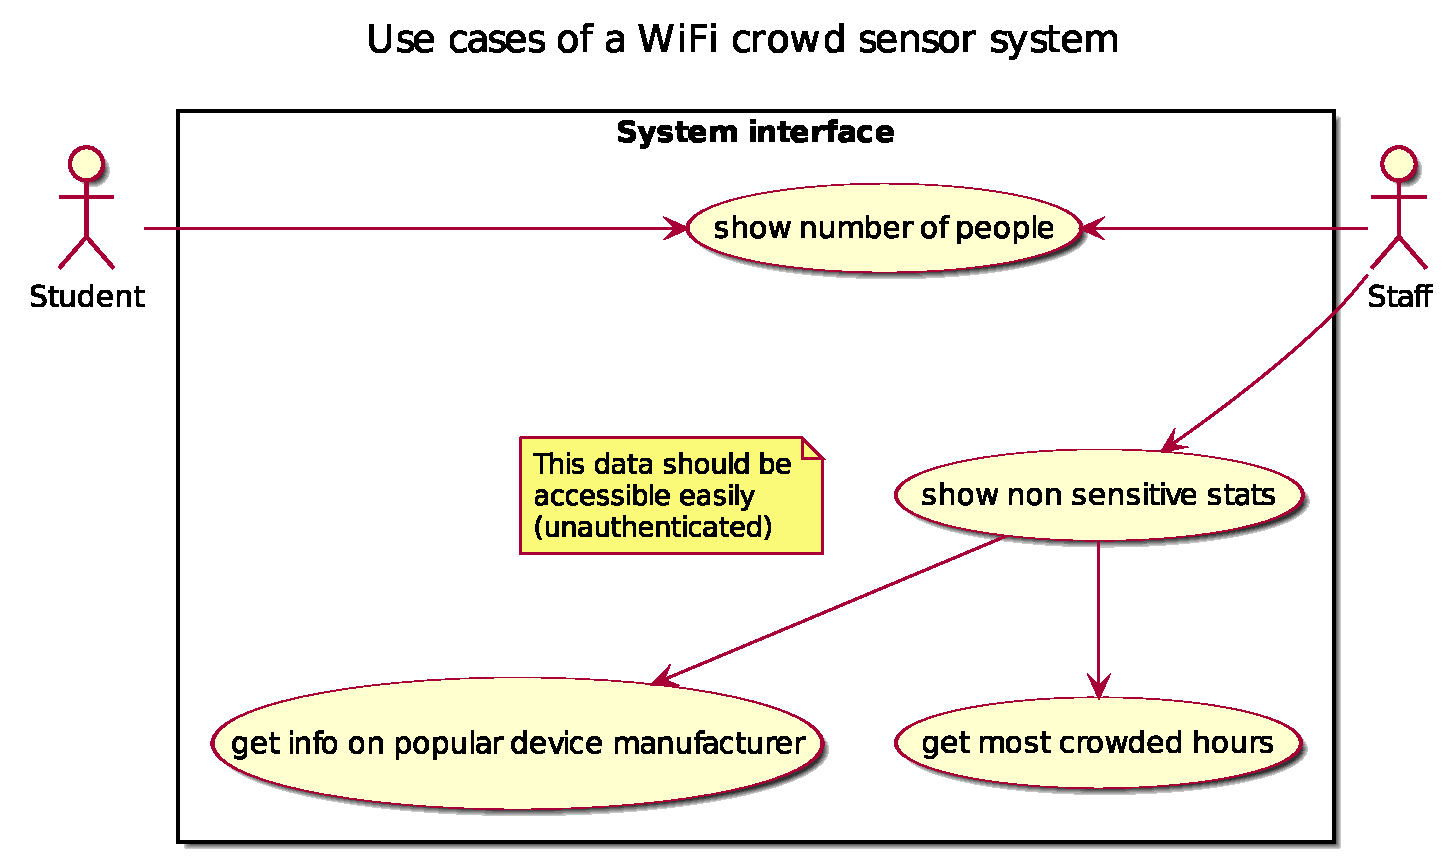
\includegraphics[width=\textwidth]{res/out/use-case.eps}
  \caption{Diagramma UML che riassme i casi d'uso del sistema}%
  \label{fig:use-cases}
\end{figure}

\subsubsection{Servizio di raccolta dati}

Il funzionamento del sistema prevede l'installazione non invasiva di sensori all'interno della struttura, presumibilmente uno per stanza;
tali sensori devono poter misurare il numero di persone all'interno delle stanze senza richiedere un contributo attivo da parte di ciascun individuo.

Un esempio può essere l'impiego di microcontrollori e/o SBC (\emph{Single Board Computer}) a basso consumo equipaggiati con un modulo WiFi in grado di lavorare in modalità promiscua.

\subsubsection{Servizio di visualizzazione dell'affollamento}

La misura dell'affollamento è il dato principale che il sistema deve raccogliere e fornire all'utente;
tale dato deve essere liberamente accessibile senza richiedere la registrazione dell'utente.
Inoltre, l'interfaccia di visualizzazione deve essere fruibile su quante più piattaforme possibile.

Tra i dati da visualizzare, è necessario mostrare:

\begin{itemize}
  \item un contatore del numero di dispositivi;
  \item un grafico rappresentante la variazione nel numero di persone nell'ultimo periodo (ad esempio, nell'ultima ora).
\end{itemize}

\subsubsection{Servizio di visualizzazione degli statistici}

Nella raccolta dei dati per il conteggio degli individui, vengono ottenute informazioni aggiuntive che possono essere considerate interessanti;
ad esempio, interecettando i pacchetti WiFi contenenti l'indirizzo MAC di ciascun dispositivo, è possibile registrare la popolarità dei vari vendor di dispositivi dotati di WiFi.

\subsection{Requisiti non funzionali}

In aggiunta ai requisiti elencati nella \Cref{subsec:req:func}, ne sono stati individuati altri di natura tecnlogica/implementativa:

\begin{description}
  \item[Semplicità di utilizzo]
    Il sistema deve risultare il quanto più possibile semplice ed intuitivo nell'utilizzo per la maggior parte degli utenti;
    ciò significa semplificare per quanto possibile le procedure per accedere alle funzionalità del sistema (ad esempio, realizzando un interfaccia web pubblicamente accessibile).
  \item[Architettura distribuita]
    Il sistema deve essere pensato per poter scalare da un ambiente ristretto composto da un singolo edificio con singola stanza ad una struttura più estesa composta da più edifici e/o più stanze;
    di conseguenza, affidarsi ad un'architettura monolitca sarebbe decisamente complicato e inefficiente.

    Per riuscire a garantire un corretto ed efficace funzionamento del sistema, occorre prendere in considerazione un'architettura distribuita e le conseguenti problematiche:

    \begin{description}
      \item[Consistenza]
        Il sistema deve riuscire a mantenere lo stato il più possibile consistente tra le repliche per supportare il carico di lavoro.
      \item[Scalabilità]
        Il sistema deve riuscire a gestire in maniera ottimale il carico a cui sottoposto.
      \item[Efficienza]
        Il sistema deve riuscire a rispondere a tutte le richieste senza tralasciarne alcuna.
    \end{description}

  \item[Privacy]
    Anche considerando le problematiche legali segnalate nella \Cref{sec:state-of-art}, la corretta anonimizzazione dei dati deve essere presa in considerazione.
  \item[Sicurezza]
    Per quanto pubblicamente \emph{consultabile}, il sistema deve permettere l'inserimento dei dati solo alle componenti autorizzate del sistema.
    In condizioni normali, non deve essere possibile per un utente umano modificare i contenuti raccolti;
    in casi eccezionali, il manutentore dovrebbe agire manualmente tramite API e con un token di autenticazione richiedibile per l'occasione.
  \item[Ingombro dei sensori e autonomia]
    Poiché il sistema non deve richiedere un'installazione invasiva, i sensori e i server locali devono essere:
    \begin{itemize}
      \item sufficientemente piccoli da poter essere nascosti in mobili già presenti nei locali senza modificazioni fisiche dell'ambiente;
      \item alimentabili in modo ``flessibile'' da batterie o da prese a muro.
    \end{itemize}
\end{description}


\newpage

%----------------------------------------------------------------------------------------
%	PROGETTAZIONE
%----------------------------------------------------------------------------------------
\section{Progettazione}\label{sec:project}

% Devono essere esposte le scelte progettuali operate nelle varie fasi di sviluppo dell'elaborato.

% In questa sezione devono essere documentati gli schemi di progetto relativamente all'architettura complessiva del sistema e alle sue componenti di rilievo.
% Per le componenti software si può ricorrere ad esempio a diagrammi delle classi, di sequenza, stato, attività.
% Per le componenti hardware è possibile includere opportuni schemi in grado di descrivere l'architettura fisica adottata.

% Vincoli circa la lunghezza della sezione (escluse didascalie, tabelle, testo nelle immagini, schemi):
% Numero minimo di battute per 2 componenti: 12000
% Numero massimo di battute per 2 componenti: 21000

In questa \nameCref{sec:project} viene presentata l'architettura generale del sistema,
partendo da come è stata derivata a partire dai requisiti raccolti, seguendo un approccio top-down:
si affronterà quindi prima la progettazione dell'architettura ad alto livello
e in un secondo momentole effettive implementazioni e architetture di dettaglio.

Il primo passo compiuto è stata la stesura del diagramma dei casi d'uso, riportato in \Vref{fig:use-cases},
\unsure{Sarà una ripetizione con quanto dico dopo?}
fondamentale per inquadrare correttamente le funzionalità da realizzare sulla base dei requisiti.

\subsection{Architettura generale del sistema}

Come detto, il punto di partenza per l'ideazione dell'architettura sono stati i casi d'uso e i requisiti non funzionali individuati in fase di analisi:
da questi ultimi emergeva infatti la necessità di creare un sistema distribuito, scalabile e allo stesso tempo di semplice accesso.

Fin da subito, è apparsa evidente l'esigenza di implementare un'architettura che potesse distinguere livello principali:

\begin{enumerate}
  \item
    un primo livello dovrebbe essere quello dei \emph{sensori IoT}, diffusi nell'ambiente (ad esempio, almeno uno per stanza);
    essi dovrebbero svolgere al massimo una minima elaborazione locale,
    in quanto appoggiarsi al livello successivo, computazionalmente più potente, permetterebbe una maggiore flessibilità sull'analisi dei dati raccolti.
  \item
    un secondo livello dovrebbe essere un qualche tipo di \emph{appliance in rete locale} (ad esempio, almeno uno per struttura),
    in grado di svolgere il ruolo di raccolta dei dati e di \emph{gateway} verso l'esterno;
  \item
    un terzo livello, più esterno, che svolge un ruolo di aggregazione ulteriore, oltre a fornire l'accesso ai dati delle strutture da reti differenti.
\end{enumerate}

Quella che siamo andati a delineare è dunque un'architettura molto simile al concetto di \textbf{Fog Computing} come descritto da Cisco~\cite{CiscoSystems2016} nella teorizzazione originale.

Definita dunque questa architettura di massima, si è delineato le entità principali del sistema:

\begin{description}
  \item[Sensori IoT]
    Il primo livello citato sopra è costituito da sensori in grado di collegarsi autonomamente col gateway tramite protocollo wireless (ad esempio, WiFi 2.4GHz).
    Nel prototipo che si intende realizzare, si intende monitorare una singola stanza e verrà utilizzato un singolo sensore;
    l'ambiente di studio, infatti, ha stanze di media grandezza, che vengono coperte ``di misura'' dalle antenne embedded nel PCB di molti sensori dotati di modulo WiFi.
  \item[Server Fog] % TODO: ricorda di sostituire edge con fog ovunque
    Il secondo livello sarà realizzato tramite un PC a basso consumo (presumibilmente basato su SoC ARM) incaricato di ospitare:
    \begin{itemize}
      \item il codice di backend per svolgere il ruolo di \emph{gateway} tra i sensori e il cloud;
      \item un'interfaccia web in grado di mostrare informazioni sull'ambiente monitorato;
      \item gli eventuali server necessari all'infrastruttura per la comunicazioni dei sensori con il backend (come ad esempio un \emph{message bus} o un \emph{publish/subscribe broker}).
    \end{itemize}
  \item[Cloud]
    Il livello cloud sarà realizzato appoggiandosi a un provider in grado di offrire:
    \begin{itemize}
      \item
        un servizio PaaS per l'hosting del codice di backend,
        preferibilmente implementato nella medesima tecnologia scelta per il livello fog, al fine di massimizzare il riuso del codice.
      \item
        un servizio PaaS per l'hosting del codice di frontend web in grado di mostrare informazioni su tutti gli edifici monitorati (nel prototipo, uno solo).
      \item
        un servizio di database gestito, possibilmente ottimizzato verso un elevato I/O\@;
        per il momento, l'essere relazionale o meno non è considerato rilevante.
    \end{itemize}
\end{description}

In \Cref{fig:architecture} è riassunto graficamente quanto descirtto sopra, oltre alle interazioni che verranno analizzate nella \nameCref{subsec:interaction} successiva.

\begin{figure}[H]
  \centering
  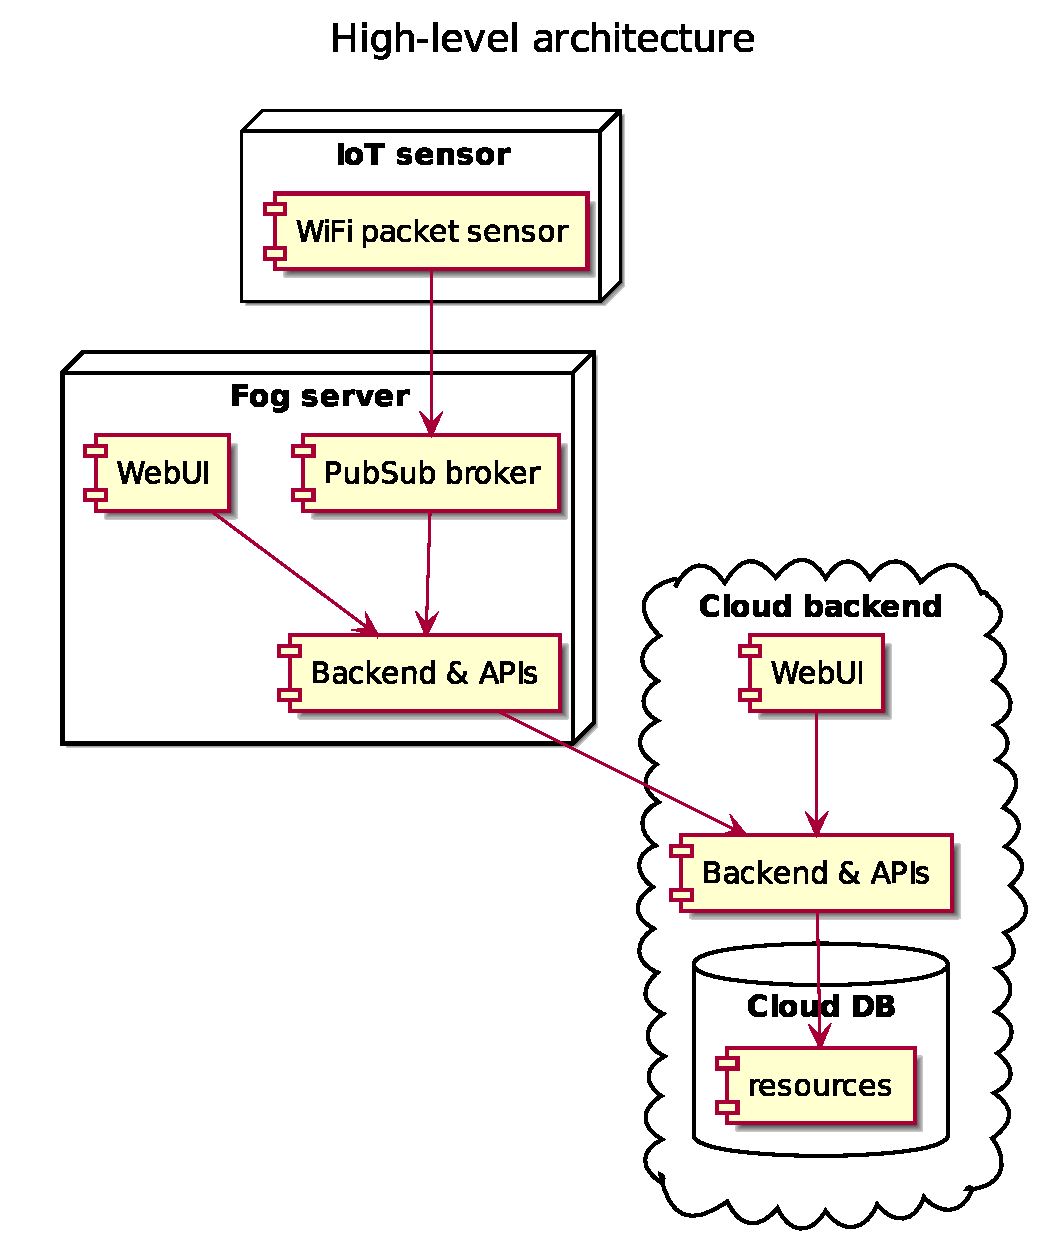
\includegraphics[width=0.7\textwidth]{res/out/architecture.eps}
  \caption{Componenti di massima dell'architettura e le loro interazioni}%
  \label{fig:architecture}
\end{figure}

\subsection{Interazioni tra gli elementi del sistema}\label{subsec:interaction}

Una volta individuate le entità fondamentali, il passo successivo è stato modellare le interazioni tra le componenti in gioco nel sistema.

Sulla base di quanto rappresentato nelle \Cref{fig:use-cases,fig:architecture}, sono stati analizzati i singoli scambi di informazioni tra le entità, analizzati come segue:

\begin{itemize}
  \item
    Per quanto riguarda la comunicazione tra il sensore e il Fog server, era necessario un protocollo di comunicazione leggero, veloce e non bloccante;
    per questi motivi, si è preferito un protocollo \emph{publish/subscribe} come MQTT~\cite{ISOCS2016}, che risulta perfetto per questi tipi di comunicazioni nell'ambito IoT.

    Per un corretto funzionamento, sarà necessario un \emph{MQTT broker} accessibile ad entrambi il Fog server e il sensore.
    Per quanto sia manualmente implementabile, si preferisce eseguire un software dedicato e indipendente;
    considerando eccessivo aggiungere un'altra macchina alla rete locale dedicata solo a questo scopo, il broker scelto verrà installato localmente al Fog server.

    In questo modo, il sensore può collegarsi al server tramite WiFi, sottoscriversi al broker come \emph{publisher}, pubblicare i dati raccolti e disconnettersi per riprendere il loop,
    mentre il backend, sottoscritto come \emph{subscriber}, si occupa di gestire quanto pubblicato.

    Si è scelto di esporre comunque API HTTP REST~\cite{Fielding2000}, che verranno utilizzate in modo asincrono dallo stesso Fog server e che permettono una espandibilità futura.
  \item
    Per quanto riguarda la comunicazione tra il Fog server e il backend in Cloud, si è ritenuto maggiormente indicato l'impiego di API REST\@.
    L'applicativo in esecuzione in cloud deve gestire le chiamate alle risorse, agendo sul database in modo asincrono e rispondendo di conseguenza.
  \item
    Per quanto riguarda le interfacce web, si è ritenuto ragionevole che il software di backend (sia Fog che Cloud) che gestisce le API possa anche servire tali pagine;
    esse, realizzate come \emph{Single Page Application}, sono in grado di risolvere le informazioni di cui hanno bisogno tramite chiamate HTTP alle API REST esposte dai rispettivi backend.
\end{itemize}

In \Cref{fig:measure} è riportato tramite diagramma UML di sequenza una rappresentazione con maggior dettaglio della procedura di registrazione di una misurazione.

\begin{figure}[H]
  \centering
  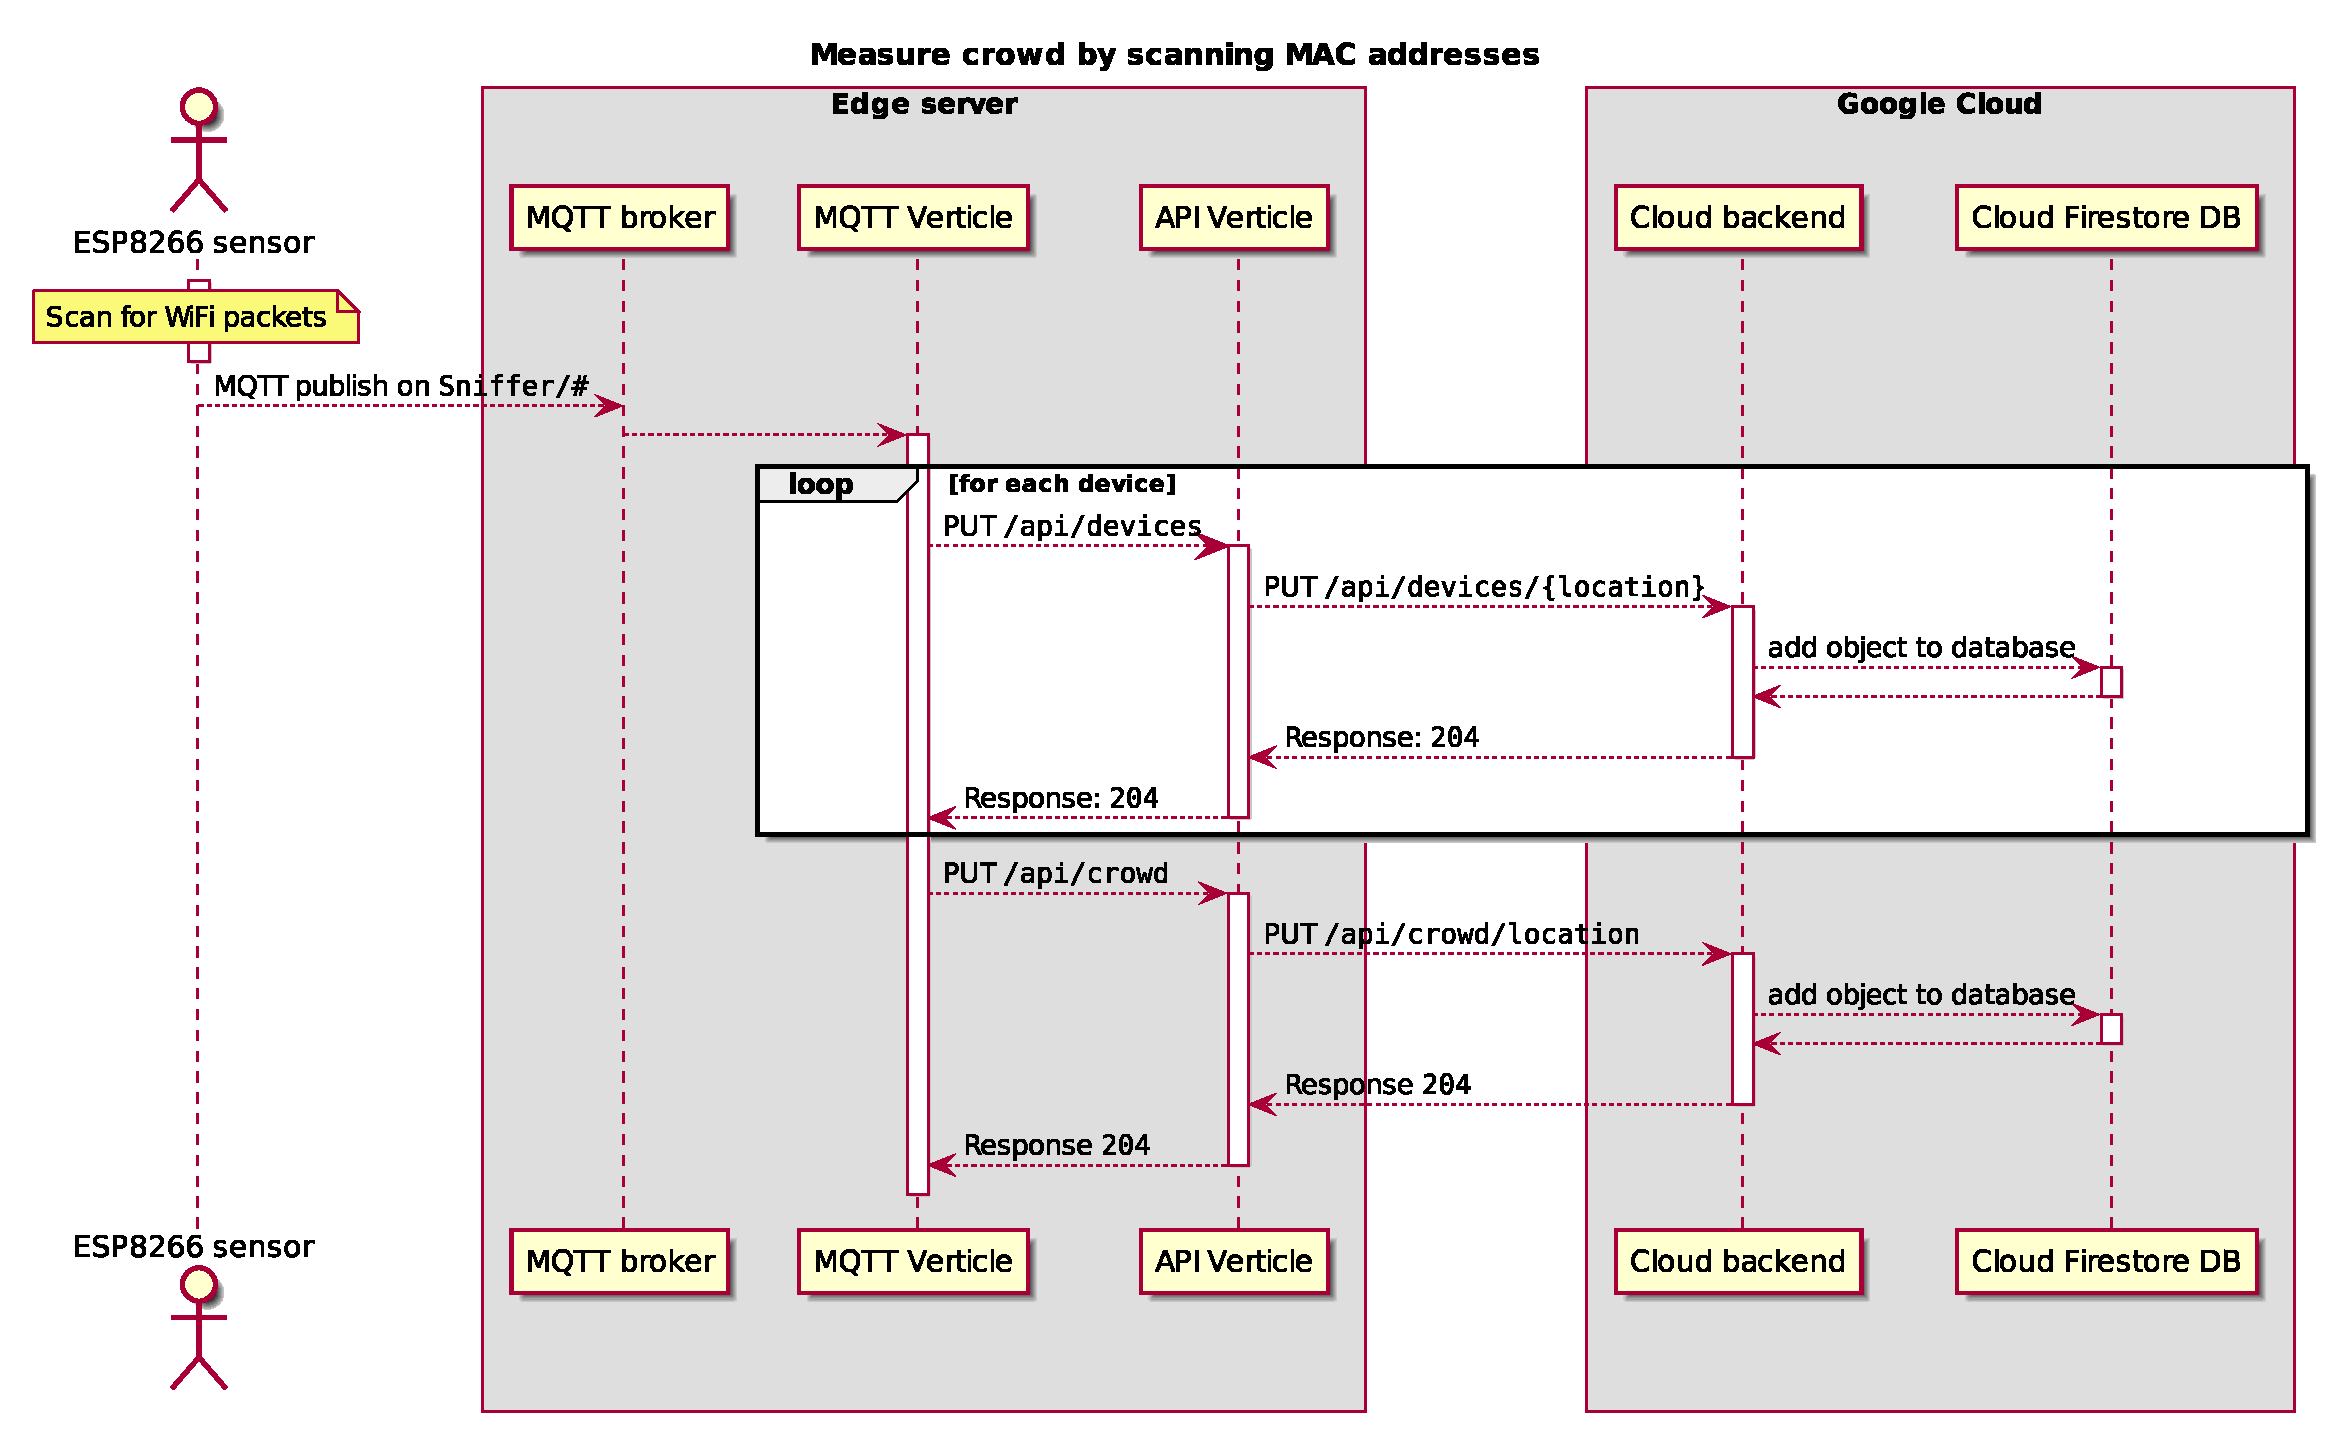
\includegraphics[width=\textwidth]{res/out/measure.eps}
  \caption{Diagramma UML di sequenza del processo di registrazione di una misurazione}%
  \label{fig:measure}
\end{figure}

\subsection{Hardware necessario}


\newpage

%----------------------------------------------------------------------------------------
%	IMPLEMENTAZIONE
%----------------------------------------------------------------------------------------
\section{Implementazione}\label{sec:implementazione}

In questa sezione verranno trattati gli aspetti inerenti all’implementazione hardware
e software legata allo sviluppo del sistema: in primo luogo saranno velocemente
presentate le tecnologie utilizzate all’interno di una o più delle entità in
gioco nel sistema, successivamente verrà dedicata una sottosezione a ciascuna di
queste dove saranno analizzate nello specifico la sua architettura e le funzionalità
di dettaglio.

\subsection{Tecnologie Utilizzate}

Di seguito sono riportate in un elenco le tecnologie più rilevanti utilizzate per l'implementazione del progetto.

\begin{description}
  \item[Typescript \& Angular: ]
    Per la realizzazione dei frontend web del server cloud e del server edge, è stato impiegato il framework Angular con il linguaggio consigliato Typescript.
    \textbf{Typescript} è un Super-set di JavaScript ES6 e, come tale, è un linguaggio di scripting orientato agli oggetti e agli eventi; Angular, invece, è un framework open source per lo sviluppo di applicazioni web con licenza MIT, evoluzione di AngularJS e sviluppato principalmente da Google.
  \item[Cloud Firestore: ]
    Per memorizzare i dati raccolti è stato utilizzato \textbf{Cloud Firestore}, un database flessibile e scalabile per lo sviluppo di dispositivi mobili, Web e server da Firebase e Google Cloud Platform.
  \item[Kotlin: ]
    Per l'implementazione di backend e gestione delle API è stato utilizzato \textbf{Kotlin}, un linguaggio di programmazione general purpose, multi-paradigma (object-oriented e funzionale), open source sviluppato dall'azienda di software JetBrains e basato su JVM.
  \item[Vertx: ]
  Libreria utilizzata all’interno dei componenti che si basano su una JVM, mette a disposizione una serie di primitive e strutture che non solo consentono di modellare un’architettura asincrona e basata sullo scambio di messaggi all’interno del singolo componente, ma permette una gestione semplice, veloce e immediata delle chiamate REST sia lato client che server.
  Tra gli altri si è optato per Vert.x, oltre che per la sua struttura basata sugli eventi asincroni all’interno di un event-loop, per la sua semplicità di deploy. A differenza di altri web server più conosciuti all’interno del mondo JVM come Java EE o Spring, Vert.x è totalmente indipendente e non necessita di un servlet container, permettendo perciò un deploy ancora più immediato.
\end{description}

\subsection{Backend Cloud}

\subsection{Frontend Cloud e Fog}

Lo sviluppo dell'interfaccia web dell'applicativo è stato realizzato attraverso il framework Angular utilizzando il linguaggio Typescript. Si è proceduto principalmente per step successivi, cercando di realizzare inizialmente uno scheletro iniziale dei vari componenti web, per poi andare a migliorare aggiungendo dettagli e features di volta in volta.

  \subsubsection{Frontend Cloud}

  L'interfaccia web per la parte Cloud consiste in una rappresentazione dei dati attraverso due grafici, entrambi realizzati grazie alla libreria \texttt{Chart.js}: uno a linee ed uno a torta.
  Il grafico a linee rappresenta l'andamento nel tempo (nell'intervallo prestabilito di 2 ore) dell'affollamento rilevato per tutti i potenziali fog (ognuno rappresentato da una linea); sull'asse delle ascisse il tempo, su quello delle ordinate il quantitativo di dispositivi trovati.
  Il grafico a torta viene utilizzato per mostrare una statistica relativa ai vari vendor (ricavabili dal MAC address) di ogni dispositivo rilevato.

  \subsubsection{Frontend Fog}

  L'interfaccia web per la parte Fog consiste in una rappresentazione tabellare dei dispositivi rilevati (comprendente vendor e un hash del MAC address per ogni dispositivo), un grafico a linee concettualmente simile a quello sviluppato nel frontend cloud ed un contatore del totale dei dispositivi trovati.

\subsection{Nodi fog}

\subsection{Sensori IoT}


\newpage

%----------------------------------------------------------------------------------------
%	TESTING E PERFORMANCE
%----------------------------------------------------------------------------------------
\section{Testing e performance}

% Esporre lo stato di funzionamento effettivo del sistema progettato ad elaborato concluso.
% Per ciascuna delle funzionalità salienti devono essere tabellate e discusse le performance riscontrate mediante opportuni test eseguiti in fase di validazione del progetto.

% I tempi di esecuzione/comunicazione devono essere accompagnati dalle caratteristiche dell'hardware sul quale è eseguito il software.

% Qualora l'elaborato includa algoritmi innovativi, indicarne la complessità computazionale (avendo cura di esporre lo pseudo codice nella sezione implementazione).

% Vincoli circa la lunghezza della sezione (escluse didascalie, tabelle, testo nelle immagini, schemi):
% Numero minimo di battute per 2 componenti: 2500
% Numero massimo di battute per 2 componenti: 4500

\subsection{Testing durante lo sviluppo}

Per quanto riguarda i piani di test, abbiamo deciso di adottare un approccio manuale:
non potendo contare su particolari framework dedicati, abbiamo realizzato la maggior parte delle prove manualmente.

\subsubsection[Backend]{Backend (Fog \& Cloud)}

Per quanto riguarda entrambi i backend, le API REST sono state testate manualmente tramite Postman\footnote{\url{https://www.getpostman.com/}}, strumento specifico per questo tipo di operazioni:
ogni volta che una nuova API veniva aggiunta al sistema, questa veniva
testata con tale strumento per verificare non solo che il server la esponesse correttamente,
ma anche che la Buisness Logic a essa collegata corrispondesse a quanto pensato in fase di progettazione.

Anche la comunicazione con il database, realizzata dopo le API, è stata testa tramite Postman, verificando dalla Firebase Cloud Console che le pubblicazioni sul DB fossero corrette.

Infine la comunicazione con MQTT, realizzata anch'essa dopo le API, è stata testata pubblicando tramite MQTT Explorer\footnote{\url{http://mqtt-explorer.com/}} rilevazioni fittizie e verificando che l'esecuzione andasse a buon fine tramite API e log.

\subsubsection[Frontend]{Frontend (Fog \& Cloud)}

Il codice relativo al frontend web è stato anch'esso testato manualmente, sia tramite server \emph{mock} quando le API non erano ancora pronte, sia con le API reali qunado disponibili.

\subsubsection{Sensori IoT}

Il codice eseguito su ESP8266 è stato anch'esso realizzato con approccio incrementale, verificando prima tramite comunicazione seriale che le rilevazioni fossero corrette, e poi via MQTT Explorer che venissero pubblicate come da aspettative.

\subsection{Testing del sistema finale}

Una volta giunti a termine dello sviluppo, si è reso necessario testare il sistema in ogni sua funzionalità.

Il sistema è stato dunque posizionato in una stanza della Biblioteca Centrale Roberto Ruffilli del Campus di Forlì per alcune ore, monitorando le rilevazioni tramite entrambe le interfacce web.

\subsubsection{Hardware utilizzato}

Per quanto riguarda l'hardware impiegato per il testing, sono state utilizzate le seguenti risorse:

\begin{itemize}
  \item
    \strong{Raspberry Pi 3 Model B} come Fog server;
    un ricevitore USB WiFi è stato collegato per poter gestire con stabilità sia la connessione \emph{upstream} ad AlmaWiFi che l'hotspot per il sensore.
    Il dispositivo è stato alimentato tramite una batteria al litio da 3700mAh.
  \item \strong{NodeMCU ESP8266} come sensore IoT, alimentato tramite un powerbank da 3350mAh.
\end{itemize}

\begin{figure}[H]
  \centering
  \begin{subfigure}[htbp]{0.45\textwidth}
    \centering
    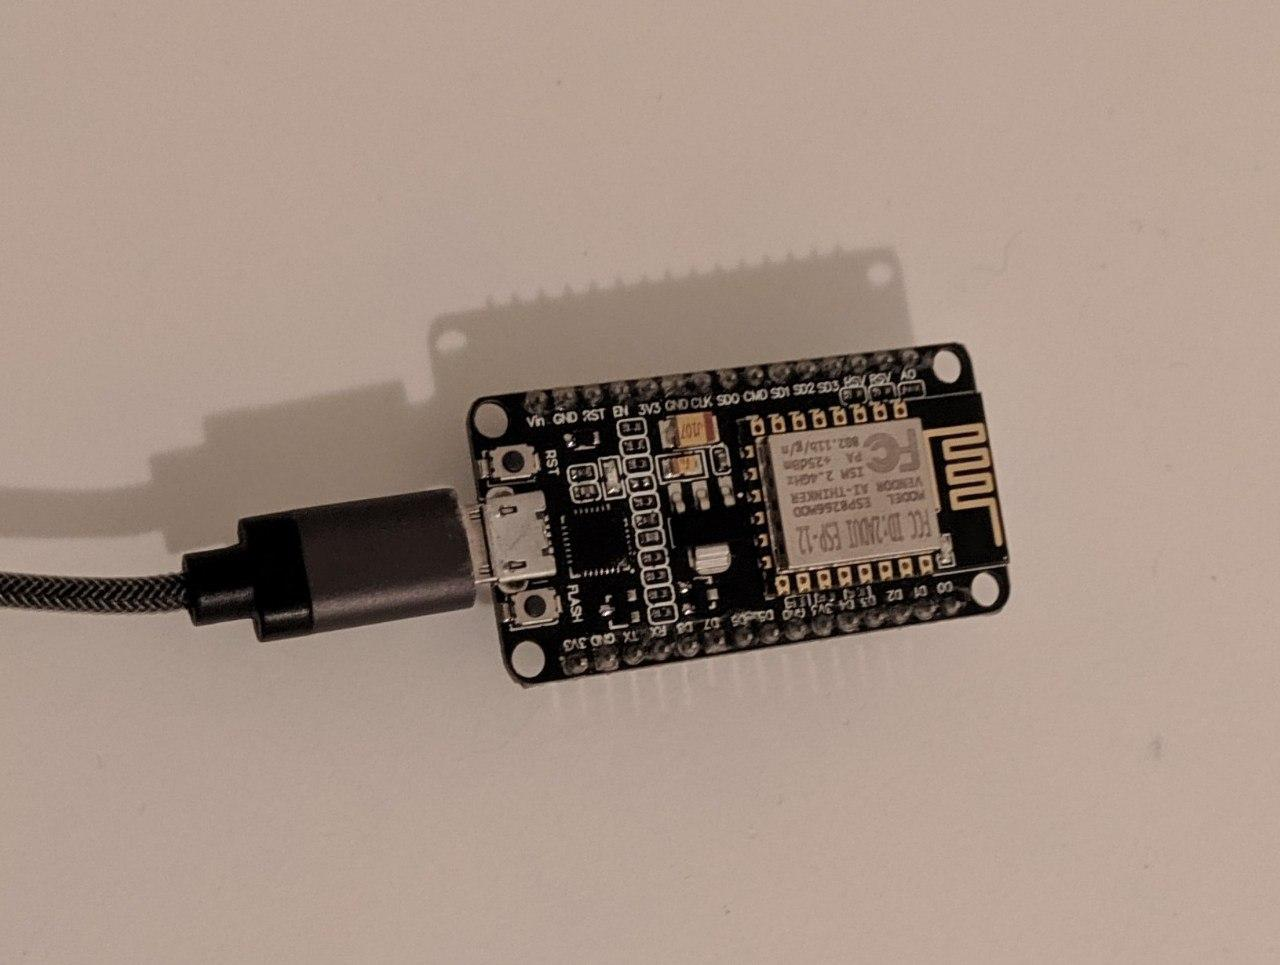
\includegraphics[width=\textwidth]{res/fig/esp.jpg}%
    \label{subfig:esp}
  \end{subfigure}
  \hfill
  \begin{subfigure}[htbp]{0.45\textwidth}
    \centering
    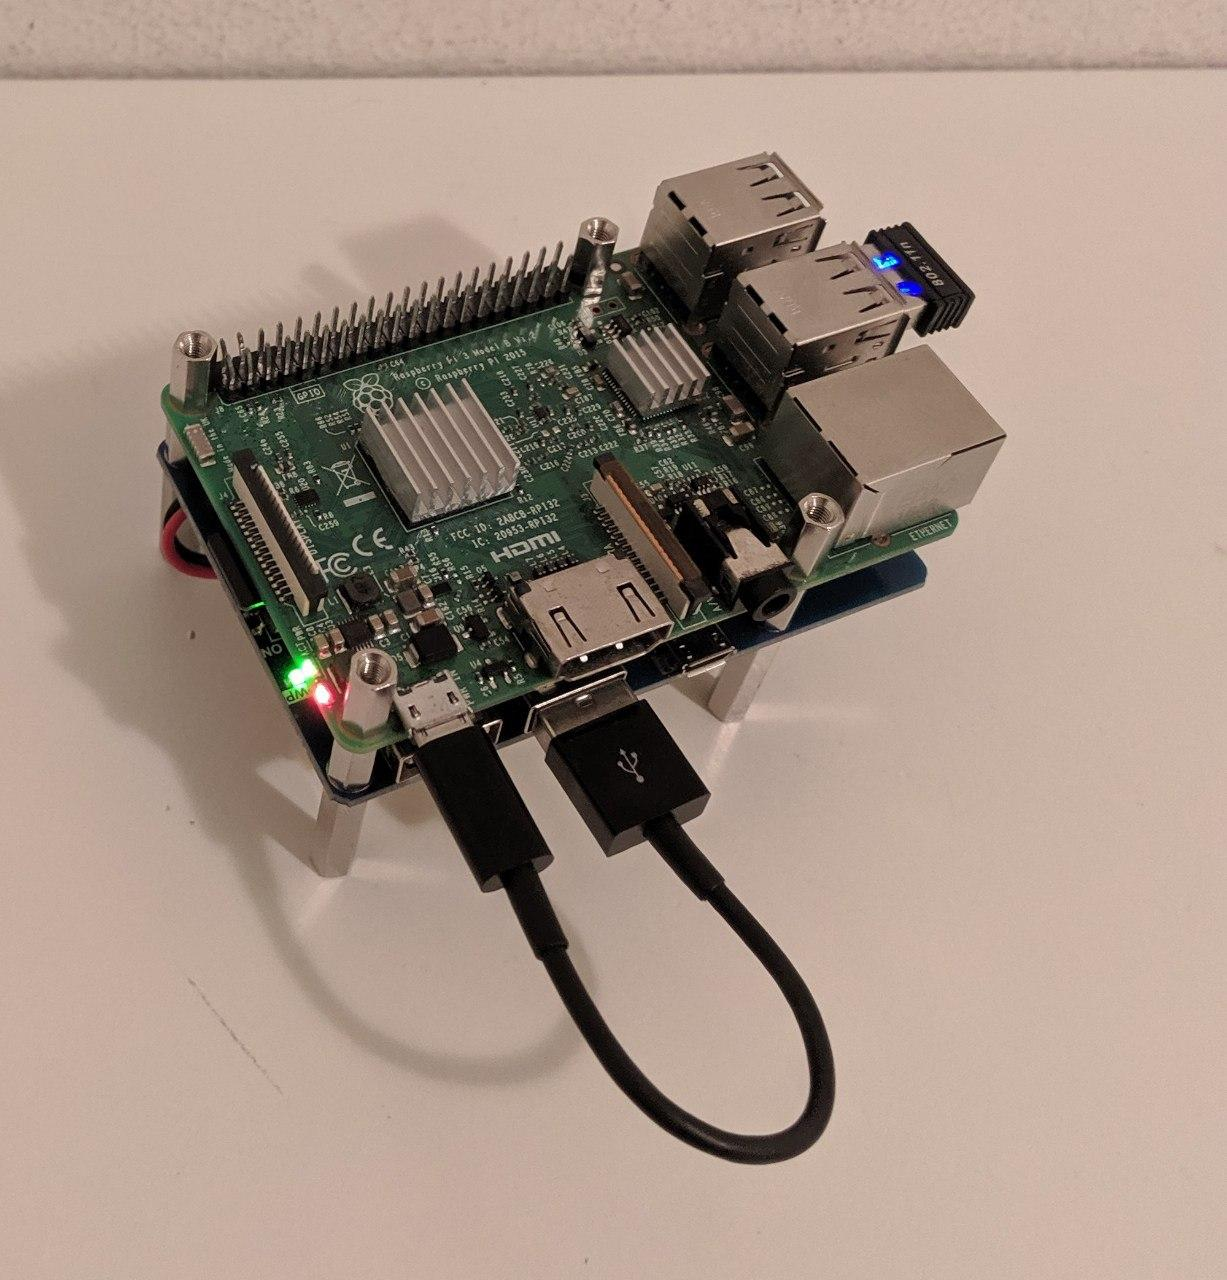
\includegraphics[width=\textwidth]{res/fig/rpi.jpg}%
    \label{subfig:raspi}
  \end{subfigure}
  \caption{Fotografie del prototipo di sistema}%
  \label{fig:hw}
\end{figure}

\subsubsection{Performance ottenute}

In questa sezione è presente una breve trattazione delle perfomance riscontrate durante il testing delle principali feature del prototipo finale:

\begin{description}
  \item[Avvio del sistema]
    Considerando i differenti sistemi:
    \begin{itemize}
      \item Il Raspberry Pi impiega generalmente circa due minuti ad avviarsi e il broker MQTT viene messo in esecuzione in pochi secondi.
      \item Il container Docker che mette in esecuzione il jar generalmente si avvia in una decina di secondi al massimo.
      \item Il sensore su ESP8266 si avvia in pochi secondi.
    \end{itemize}
  \item[Scansione delle frequenze]
    L'ESP8266 impiega in media circa 5 minuti per effettuare la scansione di tutte le 14 frequenze del WiFi supportate.
  \item[Pubblicazione su MQTT]
    L'ESP8266 impiega 5--10 secondi a collegarsi alla rete WiFi ed effettuare la pubblicazione.
  \item[Gestione delle API]
    Il Raspberry Pi e il Cloud impiegano tempi molto simili per gestire le singole chiamate API\@:
    in media, sono necessari 5--10 secondi per ottenere una risposta se è coinvolto il database, altrimenti anche meno di 5 secondi.
\end{description}


\newpage

%----------------------------------------------------------------------------------------
%	ANALISI DI DEPLOYMENT SU LARGA SCALA
%----------------------------------------------------------------------------------------
\section{Analisi di deployment su larga scala}

% In questa sezione va discussa, eventualmente con l'ausilio di opportuni diagrammi (componenti, deployment), l'evoluzione del progetto presentato immaginando che venga adottato su larga scala.
% I dettagli qui esposti devono quindi astrarre dalle specifiche dell'elaborato qualora l'implementazione sia stata focalizzata su uno scenario isolato.

% A titolo d’esempio, qualora applicabile, devono essere evidenziate le criticità che si potrebbero incontrare
% devono essere proposte soluzioni tipiche in contesti di cloud architecture per garantire un'adeguata resilienza, in termini di availability e scalability del sistema.

% Vincoli circa la lunghezza della sezione (escluse didascalie, tabelle, testo nelle immagini, schemi):
% Numero minimo di battute per 2 componenti: 6000
% Numero massimo di battute per 2 componenti: 9000

\subsection{Realizzazione reale}

Il progetto, per come è stato realizzato, costituisce un prototipo funzionante e su piccola scala di un sistema di stima di affollamento in luoghi chiusi tramite WiFi.

Per essere realmente dispiegabile, sarebbe necessario tenere in considerazione scelte hardware e software differenti, che non sono state adottate per limitazione di budget.

\subsubsection{Sensori IoT}\label{subsub:deploy:real:iot}

Per la realizzazione del prototipo di questo progetto è stato utilizzato come sensore un modulo \texttt{Espressif Systems ESP8266}\footnote{Datasheet ESP8266: \url{https://www.espressif.com/sites/default/files/documentation/0a-esp8266ex_datasheet_en.pdf}} fornito in un development kit chiamato \texttt{NodeMCU}.
Tale PCB include un modulo \texttt{ESP-12};
esso risulta adeguato per il caso di studio del prototipo, ma risulta lento nella scansione delle frequenze e le performance potrebbero peggiorare in ambienti più affollati.

Per la versione finale, l'impiego di un modulo \texttt{ESP-32}\footnote{Datasheet ESP32: \url{https://www.espressif.com/sites/default/files/documentation/esp32_datasheet_en.pdf}}
del medesimo produttore vanta un processore più veloce, un miglior ricevitore WiFi e il supporto al Bluetooth:
\begin{itemize}
  \item
    il maggior clock e il miglior ricevitore potrebbero permettere una scansione più veloce;
  \item
    il ricevitore Bluetooth potrebbe integrare il tracking anche dei pacchetti scambiati su questo protocollo per migliorare le misurazioni
    (in modo simile a quanto fatto da Waitz nel caso analizzato in \Cref{subsec:soa:waitz}).
\end{itemize}

Per aumentare ulteriormente la velocità di scansione, si potrebbero inserire un maggior numero di moduli per stanza, ciascuno impiegato solo per la scansione di un sottoinsieme delle frequenze WiFi.

\subsubsection{Connessione tra edge e cloud}

Il server edge implementato su \texttt{Raspberry Pi 3B} dipende molto dalla comunicazione con il cloud;
potrebbe essere utile collegare una scheda di rete LTE/4G/3G per fornire una connessione di rete di backup.
Inoltre, l'aggiunta di un DB locale potrebbe permettere un caching dei dati in caso di caduta della connessione fino alla risoluzione del problema.

\subsection{Deploy su larga scala}

Ragionando su un possibile deploy su larga scala del sistema, si evidenziano subito dei punti a favore e invece delle problematiche su cui riflettere.

Innanzitutto, il progetto è pensato per supportare una scalabilità sia orizzontale che verticale.
Partendo dal client web, pensando ad un numero di utenti elevato i problemi principali sono:

\begin{description}
  \item[Banda in ingresso e risorse]
    L'interfaccia web è una SPA realizzata in Angular;
    grazie a questa tecnologia, la gestione del routing, dell'ottenimento dei dati e della rappresentazione di questi ultimi è gestita client-side,
    rendendo i compiti del web server meno onerosi.

    Il server web locale potrebbe effettivamente essere limitato dalla velocità delle schede di rete del Raspoberry Pi 3B,
    il quale deve comunicare con il cloud per risolvere i dati dal database.
    L'interfaccia web dispiegata in cloud non dovrebbe essere limitata dalle risorse attualmente fornite, ma esse possono comunque essere estese \emph{on demand} in caso di necessità.

  \item[Numerosi accessi al DB]
    Come accennato nel punto precedente, il database è acceduto spesso, dunque potrebbe essere necessario l'upgrade a un piano premium (\emph{Flame} o \emph{Blaze}) per poter gestire le richieste.
\end{description}

Inoltre, il sistema molto probabilmente vedrebbe un aumento della quantità di server edge e sensori.
Infatti, come già detto nei punti precedenti, il poter aggiungere e rimuovere stanze ed edifici in modo semplice è una caratteristica del sistema.

Nonostante ciò sia dunque previsto, si potrebbero presentare alcune problematiche da gestire:
\begin{description}
  \item[Aumento del numero di sensori rispetto ai server edge]
    Per quanto molto difficile per motivi di copertura del segnale WiFi, è possibile che vi sia un elevato numero di sensori connessi al medesimo server edge che gestisce l'edificio.
    Poiché nel prototipo attuale ciascun ESP8266 si collega tramite WiFi alla rete locale generata dal Raspberry Pi usando una \texttt{netmask} di \texttt{255.255.255.0}, il numero di IP assegnabili è 255.

    Nel caso si decida di aggiungere più sensori per stanza, come ipotizzato nell \Cref{subsub:deploy:real:iot}, questo aspetto potrebbe dover essere tenuto in considerazione.
  \item[Aggiunta di server edge]
    Come specificato nella \Cref{subsub:openapi}, la comunicazione tra cloud ed edge è autenticata tramite token JWT\@.
    L'API cloud che lo genera richiede a sua volta un'autenticazione tramite nome zona e chiave, che devono essere configurate tramite file di configurazione secondo le best practice di Vert.x.
\end{description}

Da quanto si può evincere, gestendo le situazioni di carico estremo come evidenziato sopra, il sistema ha mantiene le caratteristiche che lo rendono \emph{scalabile}.
Le comunicazioni sono \emph{stateless} e sia server web che database si basano su tecnologie moderne e sono scalabili all'occorrenza, rimanendo responsivi, leggeri e dinamici.


\newpage

%----------------------------------------------------------------------------------------
%	PIANO DI LAVORO
%----------------------------------------------------------------------------------------
\section{Piano di lavoro}

\todo[inline]{Sistemare float della tabella}

\begin{table}[]
  \begin{tabular}{|c|l|l|c|}
    \hline
    \textbf{Priority} & \multicolumn{1}{c|}{\textbf{Type}} & \multicolumn{1}{c|}{\textbf{Title}} & \textbf{Points} \\ \hline
    1 & Setup & Repository Setup & 1 \\ \hline
    2 & Setup & Project Setup & 2 \\ \hline
    3 & Investigation & Crowd Tracking state of art investigation & 3 \\ \hline
    4 & Investigation & ESP sensor technology state of art investigation & 3 \\ \hline
    5 & Investigation & Best Cloud Platform choice & 1 \\ \hline
    6 & Setup & Raspberry Access Point mode configuration & 2 \\ \hline
    7 & Setup & Docker Host installation on Raspberry & 1 \\ \hline
    8 & Setup & Execute Mosquitto on Docker container & 1 \\ \hline
    9 & Setup & Configure a simple container with Vert.x Java & 1 \\ \hline
    10 & Setup & Configure Google Cloud Platform & 2 \\ \hline
    11 & Setup & Configure ESP8266 & 1 \\ \hline
    12 & Implementation & ESP8266 code library adaptation & 4 \\ \hline
    13 & Implementation & MQTT publish/subsribe interface implementation & 4 \\ \hline
    14 & Implementation & Cloud FireStore Database interface implementation & 10 \\ \hline
    15 & Implementation & API Edge implementation & 6 \\ \hline
    16 & Implementation & API Cloud implementation & 6 \\ \hline
    17 & Implementation & Web GUI edge-side implementation & 15 \\ \hline
    18 & Implementation & Web GUI cloud-side implementation & 20 \\ \hline
    19 & Implementation & Final integration testings & 8 \\ \hline
  \end{tabular}
\end{table}

Per organizzare il lavoro in team nello sviluppo del progetto è stata scelto di utilizzare
una metodologia agile organizzando le ore lavorative secondo issues prestabilite, che rappresentassero
le principali problematiche da affrontare. Il progetto è stato tracciato e mantenuto interamente su GitLab
su un repository condiviso tra i membri, in questo modo è stato possibile
lavorare in maggiore autonomia. Per la gestione delle issues è stata scelta l'interfaccia dedicata di GitLab stesso.
Circa a cadenza settimanale si è effettuato un confronto del lavoro svolto da entrambi i membri del team,
progettando e pensando ai successivi step  necessari per portare a termine il progetto.
Questa gestione è risultata più che adeguata per la
realizzazione del progetto, permettendo di procedere alla sua realizzazione senza
grossi problemi grazie ad obiettivi chiari e ad una buona suddivisione delle mansioni.

\subsection{Niccolò Maltoni}

Mi sono occupato inizialmente della ricerca per quanto riguarda le tecnologie di rilevazione dell'affollamento tramite intercettazione di pacchetti WiFi.
Ho inoltre analizzato le soluzioni cloud dei provider più famosi e, una volta selezionato Google Cloud, ho studiato i vari prodotti offerti per hosting di codice e database per selezionare quello più adeguato.
Ho poi proceduto all'implementazione del codice di backend in Vert.x sia del Fog server che del Cloud server, prima documentando le API tramite OpenAPI e poi realizzando gli \emph{handler}.
Mi sono poi dedicato allo studio del progresso raggiunto nello stato dell'arte per quanto riguarda l'impiego di ESP8266 per la cattura dei pacchetti e poi ho realizzato il codice per far lavorare il dispositivo con la parte restante del sistema.

In ultimo, con l'aiuto di Semprini, ho collaborato alla ricerca e risoluzione di bug.

\subsection{Luca Semprini}

Mi sono occupato inizialmente del setup completo del Raspberry: ho configurato la modalità Access Point, installato il Docker Host ed ho inizializzato un container su cui ho eseguito Mosquitto.
Oltre alla configurazione del Raspberry, ho curato la realizzazione dell'interfaccia web nella sua interezza: sia per la parte Cloud, che per la parte Fog; ho implementato i rispettivi grafici e tabelle e la ricezione e gestione dei dati attraverso le REST api.
Infine, nella fase di testing finale ho contribuito alla risoluzione di alcuni bug, in collaborazione con il collega Maltoni.


\newpage

%----------------------------------------------------------------------------------------
%	CONCLUSIONI
%----------------------------------------------------------------------------------------
\section{Conclusioni}

La realizzazione del progetto è stato un percorso stimolante e a tratti complesso. Ci ha permesso di lavorare come team e d’imparare varie tematiche affini all’ambito dell’IoT e delle Smart Cities.
L’esserci prefissati un obbiettivo abbastanza ambizioso ci ha portato a scontrarci con problematiche e difficoltà sia sul punto delle scelte architetturali che implementative. Abbiamo quindi dovuto in primo luogo accrescere le nostre competenze in materia, per poi prendere le scelte che abbiamo ritenuto più opportune.
Il poterci confrontare con realtà simili già esistenti ci ha permesso di definire gli obbiettivi in maniera più chiara e semplice.
Abbiamo comunque cercato di apportare la nostra impronta e utilizzare una chiave di lettura differente e che ci appartenesse. Ci riteniamo complessivamente abbastanza soddisfatti del nostro prototipo, che in quanto tale non è ancora un oggetto realmente utilizzabile nel mondo reale ma un buon modello per concretizzare l'idea alla base del progetto.

Come possibili miglioramenti e sviluppi futuri si potrebbe pensare di utilizzare un sensore più potente, o impiegarne di vari per migliorare sensibilmente la raccolta dati e aumentare la precisione delle funzionalitài.

Per una reale concretizzazione bisogna tenere conto anche degli aspetti di sicurezza, i quali, sono stati ragionati ma non completamente implementati a causa di un eccessivo aumento di complessità del progetto.


\newpage

%----------------------------------------------------------------------------------------
%	APPENDICE
%----------------------------------------------------------------------------------------
% chktex-file 26
\appendix

\renewcommand{\thesection}{\Alph{section}}
\renewcommand{\thesubsection}{A.\arabic{subsection}}

\addcontentsline{toc}{section}{Appendice}
\section*{Appendice}

% Laddove necessario è possibile avvalersi di appendici alla relazione per includere materiale di approfondimento.\\

% A titolo esemplificativo possono essere incluse le schede tecniche dei componenti adottati, la normativa di riferimento che regola un particolare dominio applicativo, ecc.

\subsection{Configurazione del Raspberry Pi}\label{app:raspi}

Si è scelto di utilizzare un modulo WiFi USB in aggiunta a quello integrato nel Raspberry Pi 3,
ma è possibile utilizzare il solo modulo WiFi integrato sia come access point che come client, pur con maggiori instabilità e minori velocità.

La procedura di adattamento dell'immagine è stata documentata in modo da poter essere riproducibile in futuro.

\begin{enumerate}
  \item
    La base dell'immagine è l'ultima versione di \textbf{Raspbian} nella sua versione minimale \textbf{lite}:
    in questo caso, la versione Buster del 26 settembre 2019.

    Dopo l'installazione, sono stati aggiornati i pacchetti tramite \texttt{apt} via rete WiFi;
  \item
    seguendo la documentazione fornita sul sito ufficiale\footnote{\url{https://raspap.com/}},
    è stato installato \textbf{RaspAP} e configurato per funzionare esclusivamente via WiFi:
    \begin{enumerate}
      \item
        \texttt{curl -sL https://install.raspap.com | bash} permette di installare RaspAP\@;
      \item
        seguendo le FAQ\footnote{\url{https://github.com/billz/raspap-webgui/wiki/FAQs\#can-i-use-wlan0-and-wlan1-rather-than-eth0-for-my-ap}}
        al file \texttt{includes/config.php} si è aggiunta \texttt{wlan1} come client interface e si è impostato nel file \texttt{/etc/dhcpcd.conf}
        \texttt{wlan0} come access point
    \end{enumerate}
    In questo modo, il dispositivo dovrebbe essere in grado di collegarsi alla rete WiFi pre-configurata e mettere a disposizione una rete con SSID ``raspi-webgui''.
  \item
    utilizzando lo script ufficiale\footnote{\url{https://github.com/docker/docker-install}} si è installato Docker;
  \item
    si è installato Java 1.8 tramite pacchetto \texttt{openjdk-8-jdk-headless};
  \item
    il broker MQTT Mosquitto viene eseguito tramite container Docker \texttt{eclipse-mosquitto}.
\end{enumerate}

\subsection{Procedura di deploy su Google App Engin in \emph{flexible environment}}\label{app:gcp}

Come detto\improvement{Inserire riferimento alla sezione corretta}, % TODO
il progetto si appoggia all'ambiente App Engine della Google Cloud Platform per l'hosting del backend cloud.

Di seguito è riportata la procedura per effettuare il deploy tramite interfaccia a linea di comando.

\begin{enumerate}
  \item
    assicurarsi di avere installato \textbf{Java} e il \textbf{Google Cloud SDK} e di essere autenticati in quest'ultimo.
  \item
    generare l'uberJar da includere nell'immagine tramite Gradle:
    \begin{minted}[autogobble]{bash}
      ./gradlew clean build shadowJar
    \end{minted}
    Verrà generato un file \texttt{build/libs/crowd-sensor-cloud-backend-all.jar}.
  \item
    nella root del sottoprogetto relativo al backend cloud, sono presenti due file:
    \begin{itemize}
      \item
        Il file \texttt{app.yaml} è la configurazione che definisce l'ambiente di esecuzione.
        \inputminted[fontsize=\footnotesize,frame=lines,linenos]{yaml}{../cloud-backend/app.yaml}
        Si è scelto di utilizzare il \emph{flexible environment} con \emph{runtime} Docker.
      \item
        Il \texttt{Dockerfile} definisce una \emph{runtime} per eseguire \texttt{verticle} di Vert.x.
        \inputminted[fontsize=\footnotesize,frame=lines,linenos]{dockerfile}{../cloud-backend/Dockerfile}
    \end{itemize}
    Tali file saranno individuati automaticamente invocando:
    \begin{minted}[autogobble]{bash}
      gcloud app deploy --project wifi-crowd-sensor-system
    \end{minted}
  \item
    Tramite il comando \mintinline{bash}{gcloud app browse} verrà aperto il link alla web UI del progetto:
    \url{http://wifi-crowd-sensor-system.appspot.com}
\end{enumerate}


\newpage

%----------------------------------------------------------------------------------------
%	RIFERIMENTI BIBLIOGRAFICI
%----------------------------------------------------------------------------------------
\printbibliography[%  % produce la bibliografia
  heading=bibintoc    % inserisce il titolo nell'indice generale
]

%----------------------------------------------------------------------------------------

\end{document}
